
\subsection{Ejercicios}
\begin{itemize}
 \item \textbf{Ejercicio 1 } Programar un tipo de tarea TaskConsola, que simulara una tarea interactiva.
La tarea debe realizar n llamadas bloqueantes, cada una de una duracion al azar 1 entre bmin
y bmax (inclusive). La tarea debe recibir tres parametros: n, bmin y bmax (en ese orden) que
seran interpretados como los tres elementos del vector de enteros que recibe la funcion.
\item \textbf{Ejercicio 2} Escribir un lote de 3 tareas distintas: una intensiva en CPU y las otras dos de
tipo interactivo (TaskConsola). Ejecutar y graficar la simulacion usando el algoritmo FCFS
para 1, 2 y 3 nucleos.
\end{itemize}

\subsection{Resultados y Conclusiones}

\subsubsection[Resolución Ejercicio 1]{Ejercicio 1}

\indent Dada la simpleza del código, optamos por mostrar nuestra implementación, en vez de comentarlo detalladamente.\\
\indent Realizamos un ciclo de i < params[0], donde utilizamos la función dada por la catedra, uso\_IO a la cual le pasamos
el pid correspondiente y un entero ciclos que es el valor random obtenido entre $bmin$ y $bmax$ 
\begin{center}
 \begin{verbatim}
                     ciclos = rand() % (params[2] - params[1] + 1) + params[1];
 \end{verbatim}

\end{center}

\indent A continuacion, el codigo mencionado:

\begin{verbatim}

                  void TaskConsola(int pid, vector<int> params) {
                       int i, ciclos;              
                       for (i = 0; i < params[0]; i++) {
                              ciclos = rand() % (params[2] - params[1] + 1) + params[1];  
                              uso_IO(pid, ciclos);
                       }
                  } 

\end{verbatim}

\subsubsection[Resolución Ejercicio 2]{Ejercicio 2}

\indent Para este punto, utilizamos el siguiente lote de tareas:
\begin{verbatim}
 
                                     TaskConsola 1 4 8
                                     TaskCPU 4
                                     TaskConsola 5 3 6

\end{verbatim}

\indent El mismo, presenta una tarea de uso intensivo $TaskCPU$ que dura unos 4 ticks, y otras dos interactivas, las cuales se
bloquean 1 y 5 ticks respectivamente con una duración de entre 4 y 8 para la primera y 3 y 6 para la segunda.\\
A continuacion, los respectivos graficos de mediciones


\vspace*{0.3cm} \vspace*{0.3cm}
  \begin{center}
 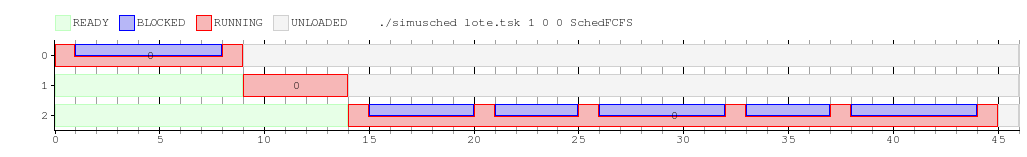
\includegraphics[scale=0.5]{ejercicio2-1nucleo.png}
 { $Lote 1$ Scheduler FCFS - 1 core }
 \end{center}
  \vspace*{0.3cm}


\vspace*{0.3cm} \vspace*{0.3cm}
  \begin{center}
 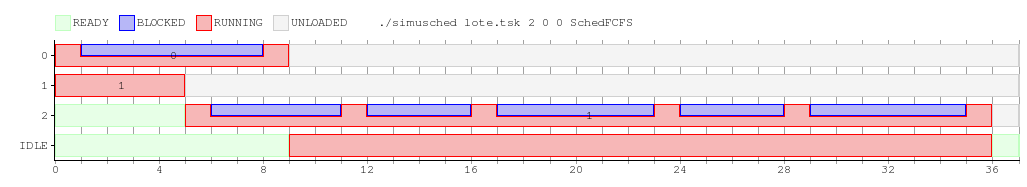
\includegraphics[scale=0.5]{ejercicio2-2nucleo.png}
 { $Lote 1$ Scheduler FCFS - 2 core }
 \end{center}
  \vspace*{0.3cm}

\vspace*{0.3cm} \vspace*{0.3cm}
  \begin{center}
 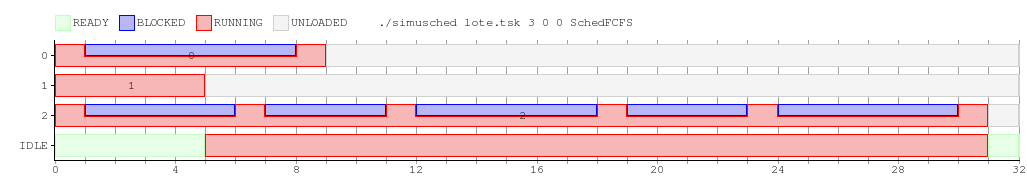
\includegraphics[scale=0.5]{ejercicio2-3nucleo.png}
  {$Lote 1$ Scheduler FCFS - 3 core }
 \end{center}
  \vspace*{0.3cm}

\indent Debido a las tareas de tipo TaskConsola, se observa que en los tres casos la duración 
de cada bloqueo es distinta.\\
\indent A modo de análisis, se puede observar por medio de los gráficos como aumenta el paralelismo a mayor cantidad de núcleos. 
En este scheduler en particular esto ayuda de gran manera al rendimiento del sistema, puesto que un nucleo podrá ejecutar otra tarea 
recién cuando haya terminado la anterior. Las consecuencias de este comportamiento son visibles en los 3 graficos. Agregando un core más, 
el tiempo que se tarda en ejecutar por completo todas las tareas de reduce casi a la mitad.\\